\PassOptionsToPackage{unicode=true}{hyperref} % options for packages loaded elsewhere
\PassOptionsToPackage{hyphens}{url}
%
\documentclass[ignorenonframetext,]{beamer}
\usepackage{pgfpages}
\setbeamertemplate{caption}[numbered]
\setbeamertemplate{caption label separator}{: }
\setbeamercolor{caption name}{fg=normal text.fg}
\beamertemplatenavigationsymbolsempty
\usepackage{lmodern}
\usepackage{amssymb,amsmath}
\usepackage{ifxetex,ifluatex}
\usepackage{fixltx2e} % provides \textsubscript
\ifnum 0\ifxetex 1\fi\ifluatex 1\fi=0 % if pdftex
  \usepackage[T1]{fontenc}
  \usepackage[utf8]{inputenc}
  \usepackage{textcomp} % provides euro and other symbols
\else % if luatex or xelatex
  \usepackage{unicode-math}
  \defaultfontfeatures{Ligatures=TeX,Scale=MatchLowercase}
\fi
\usetheme[]{CambridgeUS}
\usecolortheme{beaver}
\usefonttheme{structurebold}
% use upquote if available, for straight quotes in verbatim environments
\IfFileExists{upquote.sty}{\usepackage{upquote}}{}
% use microtype if available
\IfFileExists{microtype.sty}{%
\usepackage[]{microtype}
\UseMicrotypeSet[protrusion]{basicmath} % disable protrusion for tt fonts
}{}
\IfFileExists{parskip.sty}{%
\usepackage{parskip}
}{% else
\setlength{\parindent}{0pt}
\setlength{\parskip}{6pt plus 2pt minus 1pt}
}
\usepackage{hyperref}
\hypersetup{
            pdftitle={Daten beschaffen},
            pdfauthor={Jan-Philipp Kolb},
            pdfborder={0 0 0},
            breaklinks=true}
\urlstyle{same}  % don't use monospace font for urls
\newif\ifbibliography
\usepackage{color}
\usepackage{fancyvrb}
\newcommand{\VerbBar}{|}
\newcommand{\VERB}{\Verb[commandchars=\\\{\}]}
\DefineVerbatimEnvironment{Highlighting}{Verbatim}{commandchars=\\\{\}}
% Add ',fontsize=\small' for more characters per line
\usepackage{framed}
\definecolor{shadecolor}{RGB}{248,248,248}
\newenvironment{Shaded}{\begin{snugshade}}{\end{snugshade}}
\newcommand{\AlertTok}[1]{\textcolor[rgb]{0.94,0.16,0.16}{#1}}
\newcommand{\AnnotationTok}[1]{\textcolor[rgb]{0.56,0.35,0.01}{\textbf{\textit{#1}}}}
\newcommand{\AttributeTok}[1]{\textcolor[rgb]{0.77,0.63,0.00}{#1}}
\newcommand{\BaseNTok}[1]{\textcolor[rgb]{0.00,0.00,0.81}{#1}}
\newcommand{\BuiltInTok}[1]{#1}
\newcommand{\CharTok}[1]{\textcolor[rgb]{0.31,0.60,0.02}{#1}}
\newcommand{\CommentTok}[1]{\textcolor[rgb]{0.56,0.35,0.01}{\textit{#1}}}
\newcommand{\CommentVarTok}[1]{\textcolor[rgb]{0.56,0.35,0.01}{\textbf{\textit{#1}}}}
\newcommand{\ConstantTok}[1]{\textcolor[rgb]{0.00,0.00,0.00}{#1}}
\newcommand{\ControlFlowTok}[1]{\textcolor[rgb]{0.13,0.29,0.53}{\textbf{#1}}}
\newcommand{\DataTypeTok}[1]{\textcolor[rgb]{0.13,0.29,0.53}{#1}}
\newcommand{\DecValTok}[1]{\textcolor[rgb]{0.00,0.00,0.81}{#1}}
\newcommand{\DocumentationTok}[1]{\textcolor[rgb]{0.56,0.35,0.01}{\textbf{\textit{#1}}}}
\newcommand{\ErrorTok}[1]{\textcolor[rgb]{0.64,0.00,0.00}{\textbf{#1}}}
\newcommand{\ExtensionTok}[1]{#1}
\newcommand{\FloatTok}[1]{\textcolor[rgb]{0.00,0.00,0.81}{#1}}
\newcommand{\FunctionTok}[1]{\textcolor[rgb]{0.00,0.00,0.00}{#1}}
\newcommand{\ImportTok}[1]{#1}
\newcommand{\InformationTok}[1]{\textcolor[rgb]{0.56,0.35,0.01}{\textbf{\textit{#1}}}}
\newcommand{\KeywordTok}[1]{\textcolor[rgb]{0.13,0.29,0.53}{\textbf{#1}}}
\newcommand{\NormalTok}[1]{#1}
\newcommand{\OperatorTok}[1]{\textcolor[rgb]{0.81,0.36,0.00}{\textbf{#1}}}
\newcommand{\OtherTok}[1]{\textcolor[rgb]{0.56,0.35,0.01}{#1}}
\newcommand{\PreprocessorTok}[1]{\textcolor[rgb]{0.56,0.35,0.01}{\textit{#1}}}
\newcommand{\RegionMarkerTok}[1]{#1}
\newcommand{\SpecialCharTok}[1]{\textcolor[rgb]{0.00,0.00,0.00}{#1}}
\newcommand{\SpecialStringTok}[1]{\textcolor[rgb]{0.31,0.60,0.02}{#1}}
\newcommand{\StringTok}[1]{\textcolor[rgb]{0.31,0.60,0.02}{#1}}
\newcommand{\VariableTok}[1]{\textcolor[rgb]{0.00,0.00,0.00}{#1}}
\newcommand{\VerbatimStringTok}[1]{\textcolor[rgb]{0.31,0.60,0.02}{#1}}
\newcommand{\WarningTok}[1]{\textcolor[rgb]{0.56,0.35,0.01}{\textbf{\textit{#1}}}}
\usepackage{longtable,booktabs}
\usepackage{caption}
% These lines are needed to make table captions work with longtable:
\makeatletter
\def\fnum@table{\tablename~\thetable}
\makeatother
\usepackage{graphicx,grffile}
\makeatletter
\def\maxwidth{\ifdim\Gin@nat@width>\linewidth\linewidth\else\Gin@nat@width\fi}
\def\maxheight{\ifdim\Gin@nat@height>\textheight\textheight\else\Gin@nat@height\fi}
\makeatother
% Scale images if necessary, so that they will not overflow the page
% margins by default, and it is still possible to overwrite the defaults
% using explicit options in \includegraphics[width, height, ...]{}
\setkeys{Gin}{width=\maxwidth,height=\maxheight,keepaspectratio}
% Prevent slide breaks in the middle of a paragraph:
\widowpenalties 1 10000
\raggedbottom
\setbeamertemplate{part page}{
\centering
\begin{beamercolorbox}[sep=16pt,center]{part title}
  \usebeamerfont{part title}\insertpart\par
\end{beamercolorbox}
}
\setbeamertemplate{section page}{
\centering
\begin{beamercolorbox}[sep=12pt,center]{part title}
  \usebeamerfont{section title}\insertsection\par
\end{beamercolorbox}
}
\setbeamertemplate{subsection page}{
\centering
\begin{beamercolorbox}[sep=8pt,center]{part title}
  \usebeamerfont{subsection title}\insertsubsection\par
\end{beamercolorbox}
}
\AtBeginPart{
  \frame{\partpage}
}
\AtBeginSection{
  \ifbibliography
  \else
    \frame{\sectionpage}
  \fi
}
\AtBeginSubsection{
  \frame{\subsectionpage}
}
\setlength{\emergencystretch}{3em}  % prevent overfull lines
\providecommand{\tightlist}{%
  \setlength{\itemsep}{0pt}\setlength{\parskip}{0pt}}
\setcounter{secnumdepth}{0}

% set default figure placement to htbp
\makeatletter
\def\fps@figure{htbp}
\makeatother


\title{Daten beschaffen}
\author{Jan-Philipp Kolb}
\date{22 Oktober 2018}

\begin{document}
\frame{\titlepage}

\begin{frame}{Datenzugang}
\protect\hypertarget{datenzugang}{}

\begin{itemize}
\item
  Public-Use-File (PUF) Datei zur öffentlichen Nutzung - meist stark
  anonymisierte Daten (Beispiele:
  \href{www.forschungsdatenzentrum.de}{FDZ},
  \href{www.statistik-portal.de}{Statistik Portal},
  \href{www.infothek.statistik.rlp.de/lis/MeineRegion/index.asp}{Meine
  Region} )
\item
  Scientific-Use-File (SUF) - Datei zur wissenschaftlichen Nutzung -
  anonymisierte Daten, die zu wissenschaftlichen Zwecken und zur
  Sekundäranalyse genutzt werden können.
\item
  On-Site-Nutzung - Arbeitsplätze für Gastwissenschaftler -
  Kontrollierte Datenfernverarbeitung
\end{itemize}

\end{frame}

\begin{frame}{\href{http://inspire.ec.europa.eu/reports/Registration_form.pdf}{EU
initiative INSPIRE}}
\protect\hypertarget{eu-initiative-inspire}{}


\includegraphics{figure/inspire.PNG}

\begin{block}{Targets:}

\begin{itemize}
\tightlist
\item
  Make spatial information more accessible and interoperable -support
  sustainable development
\end{itemize}

\end{block}

\end{frame}

\begin{frame}{Zensus Atlas}
\protect\hypertarget{zensus-atlas}{}

\begin{block}{\url{https://ergebnisse.zensus2011.de/}}

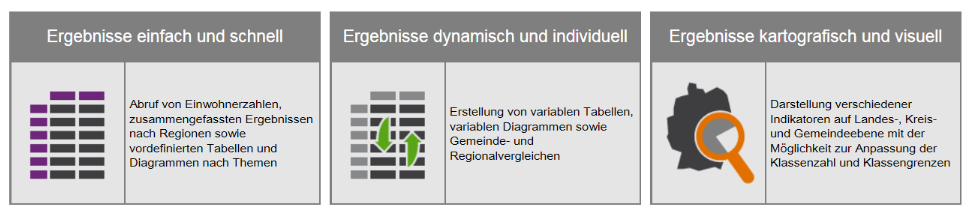
\includegraphics{figure/Zensusdtb.PNG}

\end{block}

\end{frame}

\begin{frame}{A3A Aufgabe: Zensus Ergebnisse für Gemeinden downloaden}
\protect\hypertarget{a3a-aufgabe-zensus-ergebnisse-fur-gemeinden-downloaden}{}

\begin{itemize}
\tightlist
\item
  Lade die Zensus Gemeinde Ergebniss
  \href{https://www.zensus2011.de/SharedDocs/Aktuelles/Ergebnisse/DemografischeGrunddaten.html}{\textbf{hier}}
  herunter
\item
  Importiere die Daten mit einer geeigneten Funktion
\end{itemize}

\end{frame}

\begin{frame}{\href{https://de.wikipedia.org/wiki/Amtlicher_Gemeindeschl\%C3\%BCssel}{Der
amtliche Gemeindeschlüssel}}
\protect\hypertarget{der-amtliche-gemeindeschlussel}{}

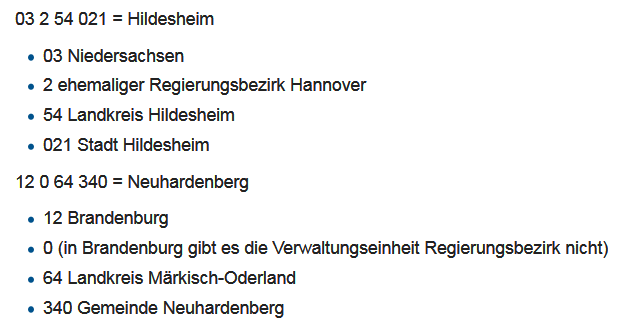
\includegraphics{figure/ags_beispiele.PNG}

\end{frame}

\begin{frame}{AGS - Bundesländer}
\protect\hypertarget{ags---bundeslander}{}

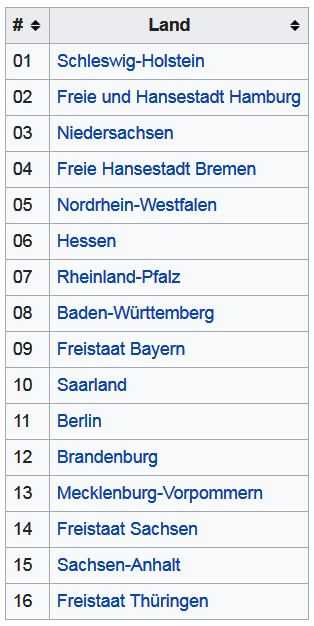
\includegraphics{figure/AGS_BLA.PNG}

\end{frame}

\begin{frame}{A3B Aufgabe}
\protect\hypertarget{a3b-aufgabe}{}

\begin{itemize}
\tightlist
\item
  Nutze die Gemeindeergebnisse für den Zensus 2011 und erzeuge einen
  Datensatz, der nur die Ergebnisse für die Saarländischen Gemeinden
  enthält.
\item
  Gib die Gemeinde an, in der der Anteil der unter 1-jährigen am
  höchsten ist.
\item
  Speichere einen Datensatz ab, in dem die folgenden Variablen enthalten
  sind:

  \begin{itemize}
  \tightlist
  \item
    der amtliche Gemeindeschlüssel,
  \item
    die Gemeindenamen,\\
  \item
    die Bevölkerungszahl insgesamt
  \item
    die Zahl der Einjährigen und
  \item
    die Zahl der Zwanzigjährigen
  \end{itemize}
\end{itemize}

\end{frame}

\begin{frame}{Forschungsdatenzentren}
\protect\hypertarget{forschungsdatenzentren}{}

\begin{itemize}
\tightlist
\item
  Bspw. FDZ der statistischen Ämter:
\end{itemize}

\url{http://www.forschungsdatenzentrum.de/}

\begin{itemize}
\item
  Es werden hauptsächlich Public Use Files angeboten,
\item
  teilweise können Gewichtungsfaktoren verwendet werden um regionale
  Ergebnisse zu bekommen
\item
  In der Regel ist Darstellung in Karten aber schwierig
\end{itemize}

\end{frame}

\begin{frame}{Weitere Amtliche Datenquellen}
\protect\hypertarget{weitere-amtliche-datenquellen}{}

\begin{itemize}
\tightlist
\item
  Genesis
\end{itemize}

\url{https://www-genesis.destatis.de/genesis/online}

\begin{itemize}
\tightlist
\item
  Daneben gibt es Angebote der Landesämter bspw:
\end{itemize}

\url{https://www.statistik.rlp.de/regionaldaten/}

\end{frame}

\begin{frame}[fragile]{Eurostat Daten}
\protect\hypertarget{eurostat-daten}{}

Sie können eine Statistik der Sparquote bei
\href{http://ec.europa.eu/eurostat/web/euro-indicators/peeis}{Eurostat}
downloaden.

\url{http://ec.europa.eu/eurostat/web/euro-indicators/peeis}

\begin{Shaded}
\begin{Highlighting}[]
\KeywordTok{library}\NormalTok{(xlsx)}
\NormalTok{HHsr <-}\StringTok{ }\KeywordTok{read.xlsx2}\NormalTok{(}\StringTok{"HHsavingRate.xls"}\NormalTok{,}\DecValTok{1}\NormalTok{)}
\end{Highlighting}
\end{Shaded}

\begin{longtable}[]{@{}llllll@{}}
\toprule
geo & X2012Q3 & X2012Q4 & X2013Q1 & X2013Q2 & X2013Q3\tabularnewline
\midrule
\endhead
Euro area (19 countries) & 9.82 & 11.86 & 11.37 & 16.28 &
10.34\tabularnewline
EU (28 countries) & 8.67 & 10.92 & 9.42 & 14.63 & 8.38\tabularnewline
Belgium & 12.52 & 9.33 & 13.99 & 19.03 & 12.07\tabularnewline
Czech Republic & 10.16 & 14.81 & 9.46 & 10.44 & 10.12\tabularnewline
\bottomrule
\end{longtable}

\end{frame}

\begin{frame}{Datahub.io}
\protect\hypertarget{datahub.io}{}

\begin{itemize}
\tightlist
\item
  Es sind sehr viele Daten vorhanden,
\item
  bspw. der UNESCO
  \href{http://datahub.io/dataset/unesco-world-heritage-sites/resource/d4116195-44d8-4bc1-9f91-9b570870dc19}{Weltkulturerbe},
  den ich in der Folge auch in Beispielen verwenden werde.
\end{itemize}

\begin{longtable}[]{@{}llrrl@{}}
\toprule
& name\_en & longitude & latitude & category\_short\tabularnewline
\midrule
\endhead
4 & Butrint & 20.03 & 39.75 & C\tabularnewline
5 & Al Qal'a of Beni Hammad & 4.79 & 35.82 & C\tabularnewline
6 & M'Zab Valley & 3.68 & 32.48 & C\tabularnewline
7 & Djémila & 5.74 & 36.32 & C\tabularnewline
8 & Timgad & 6.63 & 35.45 & C\tabularnewline
\bottomrule
\end{longtable}

\end{frame}

\begin{frame}{American Community Survey}
\protect\hypertarget{american-community-survey}{}

\begin{block}{\href{http://www.census.gov/acs/www/}{Die Daten des
\emph{American Community Survey:}}}

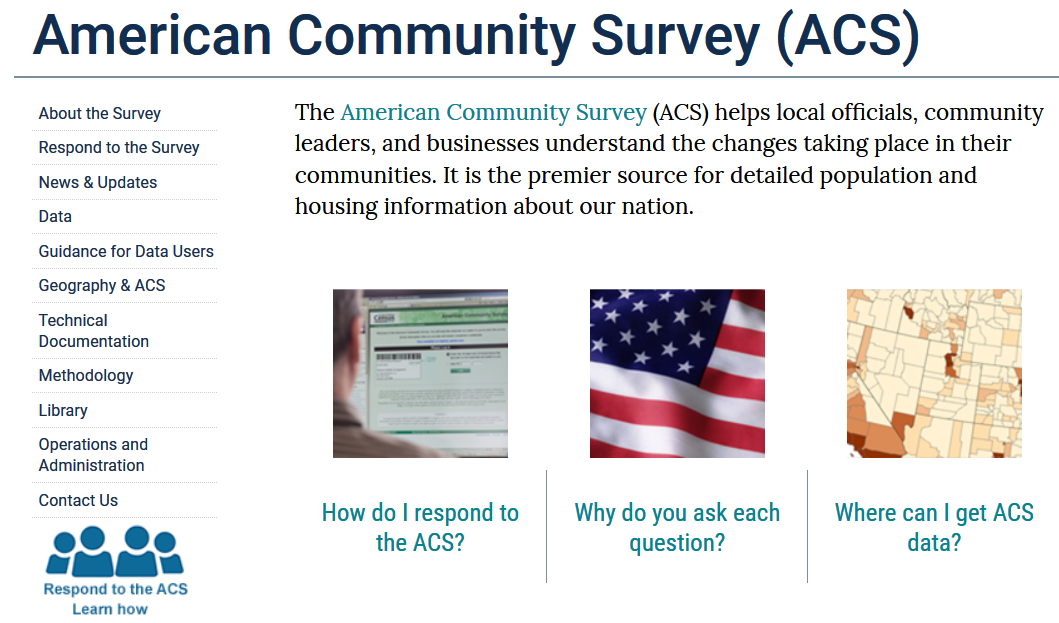
\includegraphics{figure/ACS.PNG}

\end{block}

\end{frame}

\begin{frame}{\href{data.hdx.rwlabs.org}{The Humanitarian Data
Exchange}}
\protect\hypertarget{the-humanitarian-data-exchange}{}

\begin{block}{Zum Beispiel Daten zur
\href{https://data.hdx.rwlabs.org/dataset/rowca-ebola-cases}{Ebola
Epedemie}}

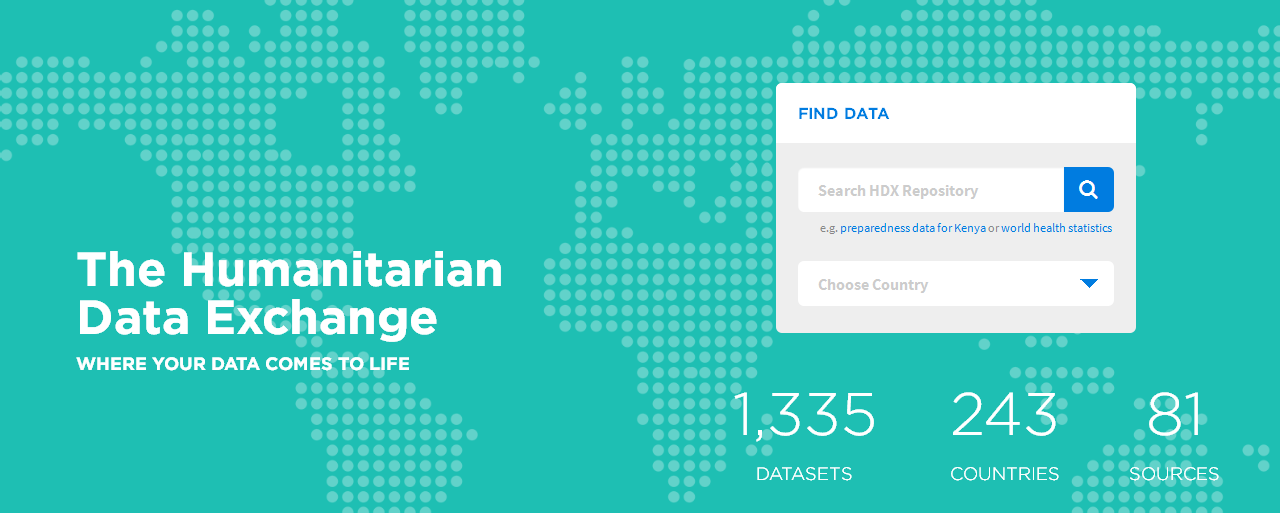
\includegraphics{figure/HDx.PNG}

\begin{itemize}
\tightlist
\item
  Zum Beispiel Ebola Fälle
\end{itemize}

\end{block}

\end{frame}

\begin{frame}{\href{http://data.london.gov.uk/dataset}{London
Datastore}}
\protect\hypertarget{london-datastore}{}

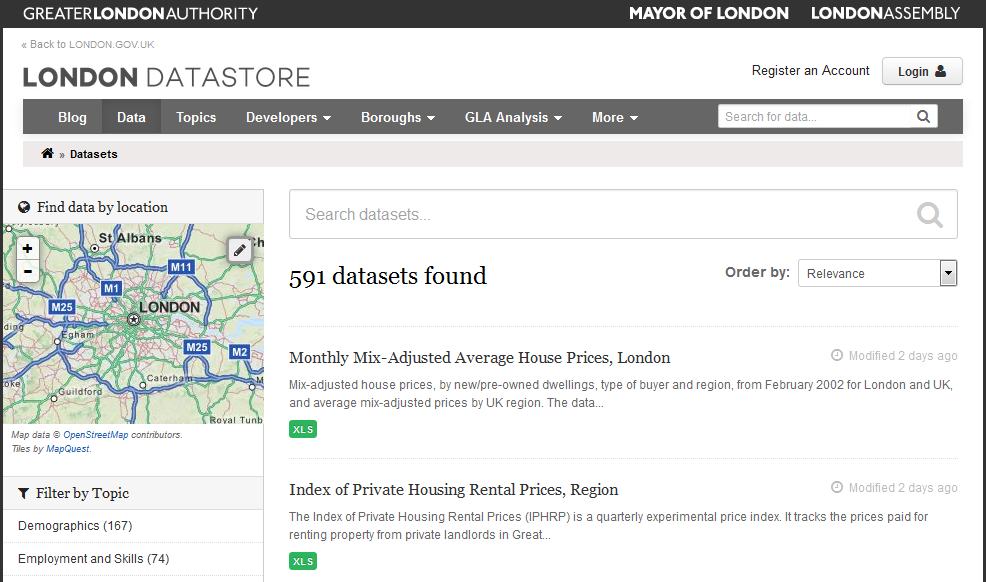
\includegraphics{figure/LondonData.PNG}

\end{frame}

\end{document}
